\documentclass[11pt,a4paper]{article}


\usepackage{amssymb,amsmath,amsfonts}    %ams
\usepackage{wasysym} %des symboles
%\usepackage{a4wide}
\usepackage[tmargin=1in,bmargin=1in,lmargin=.75in,rmargin=.75in]{geometry}
\usepackage{graphicx}
%\usepackage{pstricks}
%\usepackage{multido}
\usepackage{verbatim}
\usepackage{enumerate}
\usepackage{tikz}
\usetikzlibrary{calc,positioning,backgrounds}

\usepackage[utf8]{inputenc} 
%\usepackage[T1]{fontenc}
\usepackage{listings}

\newcommand{\R}{{\mathbb R}}   % reals
\newcommand{\Q}{{\mathbb Q}}   % rationals
\newcommand{\N}{{\mathbb N}}   %natural numbers
\newcommand{\Z}{{\mathbb Z}}    %integers
\renewcommand{\P}{{\mathbb P}}   %primes
\newcommand{\F}{{\mathbb F}}

\newcommand\cc{{\cal C}}
\newcommand{\cw}{{\cal W}}



\newtheorem{theorem}{Theorem}
\newtheorem{cor}{Corollary}
\newtheorem{example}{Example}
\newtheorem{lemma}{Lemma}
\newtheorem{newcommandi}{Definition}


\newcommand{\proof}{\noindent {\bf Proof.\ \ }}

\newcommand{\qed}{\hfill $\square$}


\newcommand{\card}[1]{\vert #1 \vert}

%\newcommand{\qed}{\hspace*{\fill} $\Box$ \bigskip }


%\renewcommand{\thefootnote}{\Alph{footnote}}
\usepackage{fancybox}
\usepackage[french]{babel}
%\usepackage{fullpage}
\usepackage{multicol}
\setlength{\columnseprule}{0.2pt}
\setlength{\columnsep}{16pt}
\usepackage{fancyhdr} % personalisation tete/pied de page
%\pagestyle{fancy}







\usepackage{hyperref}

%\addtolength{\headheight}{50pt}

\setlength{\parindent}{0pt}

\title{Fiche 3.0 : scripts et modules}
\author{BUT Informatique\\
IUT de Vélizy\\
}
\date{}


%\catcode`\_=12 %for escaping underscore

\newcommand{\ww}[1]{\textcolor{white}{#1}}

\newcommand{\code}[1]{%
    \begin{center}
        \tt #1
        \vskip .2cm
        {\tt
            \lstinputlisting[frame=single]{#1}
        }
    \end{center}
}


\usepackage{marginnote}

\usepackage{fancyvrb} % Verbatim avancé

\lstdefinestyle{customc}{
    belowcaptionskip=1\baselineskip,
    breaklines=true,
    frame=single,
    xleftmargin=2cm,
    language=C,
    showstringspaces=false,
    showspaces=false,
    basicstyle=\ttfamily
}


\newcommand{\reflexion}{\hspace{-1.2cm} 
\includegraphics[width=1cm]{reflexion.jpg} \vskip -.8cm}
%\newcommand{\checkbox}{
\includegraphics[width=.5cm]{checkbox.jpg} }
\newcommand{\checkbox}{$\square$ \smallskip}


%%environement pour les icones avec decalage
\newenvironment{icone}[1]{%
    \hskip -.8cm
\begin{tabular}{c|c}
    \hspace{.03\textwidth} \includegraphics[width=.07\textwidth]{#1} & 
\begin{minipage}{.85\textwidth}
}{%
\end{minipage}
\end{tabular}
}





\newcounter{exo} \setcounter{exo}{0}
\newenvironment{action}{%
    \begin{enumerate}[\numerotation] \addtocounter{exo}{-1}%
        }{%
    \end{enumerate}
}

%environement pour liste avec checkbox avec compteur
\newcommand{\numexoa}{\theexo \addtocounter{exo}{1}}
\newcommand{\numerotation}{\checkbox \smallskip \numexoa.}

%%environement de validation
\newenvironment{validation}{%
\smallskip
\begin{tabular}{c|c}
    \hspace{.03\textwidth} 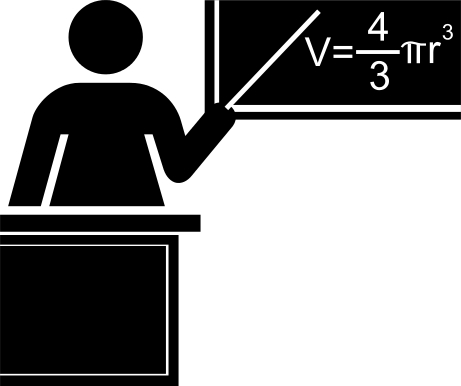
\includegraphics[width=.07\textwidth]{teacher.jpg} & 
\begin{minipage}{.85\textwidth}
}{%
\end{minipage}\\
\hline
\end{tabular}
}


%pour les fichiers c et dossiers
\newcounter{exoo} \setcounter{exoo}{0}
\newcommand{\numexo}{\theexoo}
\newcommand{\repexo}{{\tt exo\_\numexo}}
\newcommand{\exoplus}{\addtocounter{exoo}{1}}




\begin{document}
\maketitle





\thispagestyle{empty}


\section{Notion de script}

\begin{icone}{lecture.jpg}
Jusqu'à présent, vous avez écrit du python dans l'environnement interactif {\it jupyter}. Mais en général les programmes python sont indépendants de ce genre d'environnement et peuvent être exécutés "directement".

Un {\it script} python est simplement un fichier texte, dont l'extension est en général {\tt .py} et qui contient du code. Un programme python est en général un ensemble de scripts.

	En python, un script s'appelle un {\it module}, il y a quelques nuances mais ça ira pour l'instant. Plus de détails dans \url{https://docs.python.org/fr/3/tutorial/modules.html}

Pour écrire un tel script, on peut utiliser un simple {\it éditeur de texte} (gedit, vim, emacs, geany, sublimetext,...) ou un {\it environnement de développement intégré} (IDE) (eclipse, pycharm, jetbrains,vscode,...), qui est un éditeur de texte avec de nombreuses fonctions supplémentaires pour écrire du code.

Dans cette séquence, afin de ne pas tout mélanger, nous utiliserons l'éditeur {\bf geany} qui est très simple. Par la suite, vous ferez comme vous voudrez.
\end{icone}


\section{Prise en main}

\begin{action}
\item Ouvrez l'éditeur de texte {\it geany}. Tapez quelques lignes de code dans l'éditeur, par exemple effectuez une boucle pour écrire 10 fois "bonjour".
\item Enregistrez dans votre dossier de la sequence3 ce programme sous le nom {\tt first\_script.py}
\item Maintenant, ouvrez un terminal et naviguez en ligne de commande jusqu'à vous trouver dans le répertoire où se trouve le script.
\item Tapez dans la ligne de commande

	\begin{center}
		\tt python3  first\_script.py
		\end{center}
N'oubliez pas que la touche TAB permet de compléter automatiquement. En principe, vous devriez voir dans le terminal la sortie de votre programme. Sinon, c'est peut-être que vous avez un message d'erreur.
\item Retenez la procédure ci-dessus, il faudra toujours la faire pour exécuter les programmes python.
\end{action}

\section{Ecriture d'une librairie pour gérer les trucs à faire}

\begin{icone}{lecture.jpg}
	Quand vous exécutez le script, python va tout lire et exécuter, dans l'ordre du script, de haut en bas. Quand python tombe sur la définition d'une fonction,({\tt def ...}  il n'exécute pas le code de la fonction, il prend juste note de son existence. Pour vraiment exécuter la fonction, il faut l'appeler !
\end{icone} \\


Vous allez maintenant réaliser un petit module avec quelques fonctions ayant pour but de gérer une liste de tâches à réaliser ou {\tt todolist}. Plus précisément, on veut avoir en mémoire un ensemble de tâches à réaliser comme :

\begin{verbatim}
Tâches priorité haute :
	- réviser cours dev
	- appeler Mamie
Tâches priorité moyenne :
	- vaisselle
Tâches priorité basse :
	- finir de regarder F&F 42
	- réviser encore cours dev
\end{verbatim}

Vous pouvez imaginer autre chose et faire des variations plus avancées sur ce principe (possibilité de prévoir des tâches à des dates fixées, etc.)

\begin{action}
\item Créez deux scripts, {\tt todolist.py} et {\tt test\_todo.py}. Le premier contiendra l'ensemble des fonctions pour manipuler la todolist mais pas de code qui s'exécute directement, et le second les tests. Vous n'exécutez jamais le premier directement, vous exécutez le module de test qui lui se servira des fonctions écrites dans l'autre.
\item A vous de décider comment vous allez gérer la sauvegarde des tâches et leur priorité. Créez une fonction qui affiche l'ensemble des tâches comme ci-dessus. Bien entendu, vous écrivez la spécification de la fonction.
\item Dans votre fichier de tests, qui doit se trouver dans le même répertoire, écrivez {\tt import todolist} avant votre code. Ecrivez maintenant une fonction de test de votre affichage et appelez-la.
\item Maintenant, à chaque fois vous devez écrire la fonction, sa spécification, et la fonction de test. De préférence, d'abord la fonction de test. Créez une fonction pour ajouter une tâche. Attention, je n'ai pas dit saisir une tâche au clavier.
\item Ecrivez aussi des fonctions pour supprimer une tâche, ou pour archiver une tâche déjà effectuée, pour changer la priorité d'une tâche, et toute autre fonction que vous pourrez imaginer qui pourrait servir dans votre librairie.

\item Ecrivez un test complet de votre librairie : cela crée une todolist, ajoute quelques tâches, les affiche, supprime et ajoute d'autres tâches, affiche, etc.
\end{action}




\end{document}
